%%%%%%%%%%%%%%%%%%%%%%%%%%%%%%%%%%%%%%%%%%%%%%%%%%%%%%%%%%%
% --------------------------------------------------------
% Tau
% LaTeX Template
% Version 2.3.1 (10/04/2024)
%
% Author:
% Guillermo Jimenez (memo.notess1@gmail.com)
%
% License:
% Creative Commons CC BY 4.0
% --------------------------------------------------------
%%%%%%%%%%%%%%%%%%%%%%%%%%%%%%%%%%%%%%%%%%%%%%%%%%%%%%%%%%%
% --------------------------------------------------------
%     BIBLIOGRAPHY WITH BIBLATEX IN EXTERNAL EDITORS
% --------------------------------------------------------
% If the bibliography does not show up, try running the
% 'tau.cls' and 'tau.bib' file with biber from the
% MikTeX console or your preferred LaTeX distribution to
% generate the auxiliar files and (re)run the main.tex.
% --------------------------------------------------------
%%%%%%%%%%%%%%%%%%%%%%%%%%%%%%%%%%%%%%%%%%%%%%%%%%%%%%%%%%%
% --------------------------------------------------------
%					  FOR SPANISH BABEL
% --------------------------------------------------------
% \usepackage[spanish,es-nodecimaldot,es-noindentfirst]{babel}
% --------------------------------------------------------
%%%%%%%%%%%%%%%%%%%%%%%%%%%%%%%%%%%%%%%%%%%%%%%%%%%%%%%%%%%

\documentclass[9pt,a4paper,twoside]{tau}
\usepackage[english]{babel}
\usepackage{tauenvs}

%----------------------------------------------------------
% TITLE
%----------------------------------------------------------

\title{\textit{Minigrid} -- \textit{Door Key} -- Uma análise de modelos (DQN x PPO)}

%----------------------------------------------------------
% AUTHORS, AFFILIATIONS AND PROFESSOR
%----------------------------------------------------------

\author{Giancarlo Vanoni Ruggiero}
\author{Luciano Felix Dias}
\author{Tales Ivalque}

%----------------------------------------------------------

\affil{Engenharia da Computação, INSPER}

\professor{Prof. Fabrício Barth}

%----------------------------------------------------------
% FOOTER INFORMATION
%----------------------------------------------------------

\institution{INSPER}
\ftitle{}
\date{10 de maio de 2024}
\course{Reinforcement Learning}

%----------------------------------------------------------
% ABSTRACT
%----------------------------------------------------------

\begin{abstract}
    Neste projeto foi desenvolvido e validado um agente capaz de atuar no ambiente Door Key. O método de treinamento empregado foi modificar o ambiente para receber recompensas em estágios intermediários, como abrir a porta e pega a chave. Os resultados obtidos foram que utilizando o DQN o agente não foi capaz de aprender, enquanto com o PPO e com as modificações no ambiente, o agente conseguiu aprender.
\end{abstract}

%----------------------------------------------------------

\keywords{Reinforcement Learning, DQN, PPO, Minigrid, Door Key}

%----------------------------------------------------------

\begin{document}

\maketitle
\thispagestyle{firststyle}
\tauabstract
%	\tableofcontents

%----------------------------------------------------------

\section{Introdução}

\taustart{O} projeto tem como objetivo comparar o desempenho do ambiente single-agent
\href{https://minigrid.farama.org/environments/minigrid/DoorKeyEnv/}{Minigrid -- Doorkey}
utilizando os algoritmos DQN (\textit{Deep Q-Network}) e PPO (\textit{Proximal Policy Optimization}). Neste ambiente, há uma chave que o agente deve adquirir para destrancar uma porta e chegar ao objetivo no quadrado verde.

\section{Ambiente}

\begin{table}[htbp]
    \caption{Direções do espaço de observação}
    \label{tab:directions}
    \centering
    \begin{tabular}{cc}
        \toprule
        \textbf{ID} & \textbf{Vetor direção} \\
        \midrule
        0           & \(( 1,  0)\)           \\
        1           & \(( 0,  1)\)           \\
        2           & \((-1,  0)\)           \\
        3           & \(( 0, -1)\)           \\
        \bottomrule
    \end{tabular}
\end{table}

O espaço de observação é descrito por um dicionário contendo a direção do agente \textit{direciton}, a imagem observável \textit{image} e o espaço de missão \textit{mission}. Sendo: \textit{direction} um atributo discreto de valor como descrito na tabela \ref{tab:directions}; \textit{image} sendo uma matriz RGB quadrada de valores inteiros contidos no intervalo \([0, 255]\) do tamanho do campo de visão do agente, e sendo este parametrizável como numero inteiro ímpar maior que 2 por padrão 7; e \textit{mission} sendo o universo de ação do agente como uma matriz retangular de tamanho arbitrário contendo trincas seguindo a seguinte estrutura, respectivamente:

\begin{table}[htbp]
    \caption{Objetos do espaço de observação}
    \label{tab:objects}
    \centering
    \begin{tabular}{ccl}
        \toprule
        \textbf{ID} & \textbf{Nome}   & \textbf{Objeto} \\
        \midrule
        0           & \textit{UNSEEN} & Não visível     \\
        1           & \textit{EMPTY}  & Vazio           \\
        2           & \textit{WALL}   & Parede          \\
        3           & \textit{FLOOR}  & Chão            \\
        4           & \textit{DOOR}   & Porta           \\
        5           & \textit{KEY}    & Chave           \\
        6           & \textit{BALL}   & Bola            \\
        7           & \textit{BOX}    & Caixa           \\
        8           & \textit{GOAL}   & Objetivo        \\
        9           & \textit{LAVA}   & Lava            \\
        10          & \textit{AGENT}  & Agente          \\
        \bottomrule
    \end{tabular}
\end{table}

\begin{table}[htbp]
    \caption{Cores do espaço de observação}
    \label{tab:colors}
    \centering
    \begin{tabular}{ccl}
        \toprule
        \textbf{ID} & \textbf{Nome}   & \textbf{Vetor RGB}  \\
        \midrule
        0           & \textit{RED}    & \((255, 0, 0)\)     \\
        1           & \textit{GREEN}  & \((0, 255, 0)\)     \\
        2           & \textit{BLUE}   & \((0, 0, 255)\)     \\
        3           & \textit{PURPLE} & \((112, 39, 195)\)  \\
        4           & \textit{YELLOW} & \((255, 255, 0)\)   \\
        5           & \textit{GREY}   & \((100, 100, 100)\) \\
        \bottomrule
    \end{tabular}
\end{table}

\begin{table}[htbp]
    \caption{Estados do espaço de observação}
    \label{tab:states}
    \centering
    \begin{tabular}{ccl}
        \toprule
        \textbf{ID} & \textbf{Nome}   & \textbf{Estado} \\
        \midrule
        0           & \textit{OPEN}   & Aberto          \\
        1           & \textit{CLOSED} & Fechado         \\
        2           & \textit{LOCKED} & Trancado        \\
        \bottomrule
    \end{tabular}
\end{table}

\begin{table}[htbp]
    \caption{Espaço de ação}
    \label{tab:actions}
    \centering
    \begin{tabular}{ccl}
        \toprule
        \textbf{Número} & \textbf{Nome}    & \textbf{Ação}             \\
        \midrule
        0               & \textit{LEFT}    & Vira para a esquerd       \\
        1               & \textit{RIGHT}   & Vira para a direita       \\
        2               & \textit{FORWARD} & Move para a frente        \\
        3               & \textit{PICKUP}  & Pega um objeto            \\
        4               & \textit{DROP}    & Não utilizado             \\
        5               & \textit{TOGGLE}  & Alternar/ativar um objeto \\
        6               & \textit{DONE}    & Não utilizado             \\
        \bottomrule
    \end{tabular}
\end{table}

O espaço de ação é discreto com ações de movimento e poucas interações com elementos do ambiente. O espaço de ação é implementado conforme especificado na tabela \ref{tab:actions}.

A função de recompensa é definida no domínio contínuo do intervalo \([0, 1]\) e proporcional a razão entre o número de passos e o número máximo de passos permitido para o agente atingir o estado final com sucesso, caso contrário a recompensa é anulada. Esta razão é definida com maior rigor na equação \ref{ec:equation}.

\begin{equation}
    \label{ec:equation}
    \text{RECOMPENSA} =
    \begin{dcases}
        1-0.9\cdot\frac{\text{\#PASSOS}}{\text{max(\#PASSOS)}}, & \text{se sucesso}     \\
        0,                                                      & \text{caso contrário}
    \end{dcases}
\end{equation}


\section{Método}

Para conseguir comparar bem o desempenho dos dois algoritmos no ambiente, será analisado o crescimento da recompensa de um agente treinado em cada um desses algoritmos, utilizando a MlpPolicy, e 200.000 passos de aprendizado. O ambiente utilizado dentro do Minigrid - Doorkey será o "MiniGrid-DoorKey-6x6-v0", que já oferece uma complexidade razoável para o agente. Mas, para obter uma comparação satisfatória, é necessário primeiramente alterar a função recompensa de modo a ficar mais nítido o aprendizado de cada agente.

\begin{info}[frametitle=Atenção]
    Para treinamento será utilizado a biblioteca \textit{stable baselines}.
\end{info}

Inicialmente, para conseguir utilizar a biblioteca \textit{stable baselines}, foi necessário utilizar do \textit{ImgObsWrapper}, que é um \textit{Wrapper} específico do ambiente, que transforma a observação do \textit{environment} em um formato de Imagem, próprio para interpretação da biblioteca. Junto a isso, foi necessário utilizar dois outros \textit{Wrappers} que alterassem a recompensa entregue ao agente para que o treinamento pudesse ser realizado e analisado. Desses, um é o \textit{PositionBonusWrapper}, que também é específico do ambiente \textit{Minigrid} e permite a recompensa da exploração do agente, o outro é um \textit{Wrapper} original feito pela equipe de forma para recompensar as ações intermediárias antes de chegar ao objetivo final.

O \textit{Wrapper} orignal implementado tem o seguinte funcionamento:
\lstinputlisting[caption=Código do Wrapper, language=python]{assets/CustomRewardWrapper.py}

Agora, a função recompensa é definida no domínio contínuo do intervalo [-0.25, 3], levando em conta as ações pegar a chave e destrancar a porta, além de punir o número de passos do agente, isso na sua primeira parcela. O \textit{PositionBonusWrapper} provê uma segunda parcela inversamente proporcional à raiz do número de vezes que uma determinada posição foi visitada. O cálculo da recompensa final pode ser visto nas equações \ref{ec:equation2} e \ref{ec:equation3}.

\begin{equation}
    \label{ec:equation2}
    \text{NEW REWARD} =
    \begin{dcases}
      -0.1,                      & \text{Por cada step}                       \\
        0.5,                        & \text{Pegar a chave ou destrancar a porta}     \\
        -0.25,                      & \text{Caso feche uma porta}                       \\
        2,                          & \text{Ao chegar ao destino final}
    \end{dcases}
\end{equation}

\begin{equation}
    \label{ec:equation3}
   \text{NEW REWARD} +\!= \frac{1}{\sqrt{\text{\#VISITAS}}}
\end{equation}

Após a configuração dos rewards, vem a etapa de treinamento dos agentes. O setup é feito da seguinte maneira para o agente DQN:
\lstinputlisting[caption=Modelo DQN, language=python]{assets/train_dqn.py}
E para o modelo PPO:
\lstinputlisting[caption=Modelo PPO, language=python]{assets/train_ppo.py}

\section{Resultados}

Através dos treinamentos foi possível obter a curva de aprendizagem mostrada na Figura \ref{fig:figure}. Através dela é possível notar que após 100000 episódios o PPO consegue convergir, o DQN não converge em nenhum momento. Também é possível notar que o \textit{reward} começa alto em ambos e vai decaindo, até se estabilizar.

\begin{figure}[htbp]
    \centering
    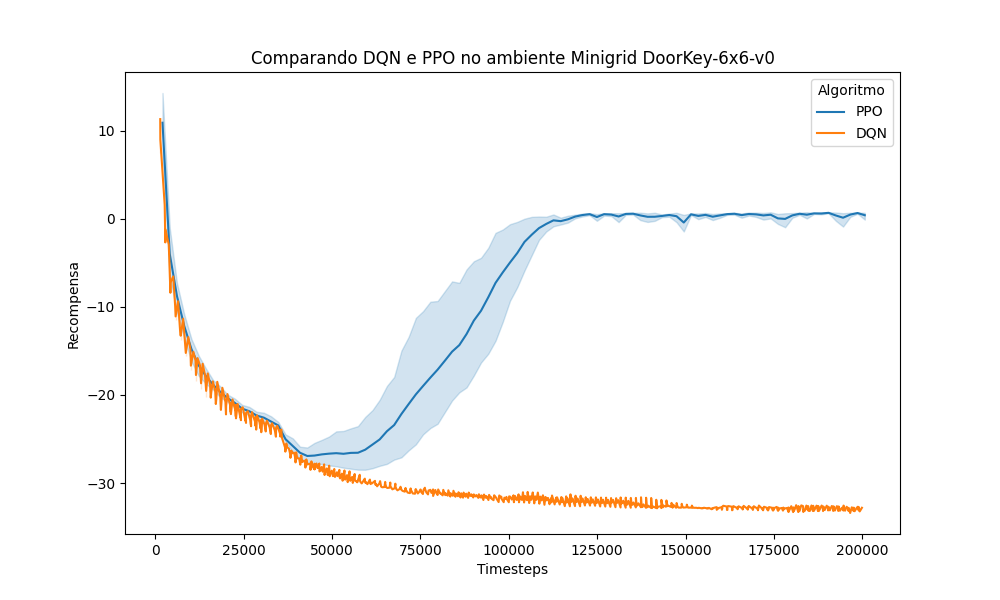
\includegraphics[width=0.8\columnwidth]{assets/plot.png}
    \caption{Curva de aprendizado MiniGrid-6x6-v0, comparando DQN e PPO}
    \label{fig:figure}
\end{figure}

Outro resultado que encontramos foi que mesmo treinando no ambiente 6x6 o treinamento funcionou no ambiente 8x8. Isso se deve ao fato de que como o ambiente não é totalmente observável o agente aprendeu a procurar os objetos para chegar em seu objetivo.

\section{Considerações finais}

\taustart{O} objetivo deste trabalho foi explorar o ambiente \textit{Minigrid-Doorkey}, que possui características únicas, como o fato de ter um espaço de observação limitado e também depender de aleatoriedade, já que originalmente o agente só iria receber recompensa caso chegasse no final. Ao longo do desenvolvimento foi possível modificar o ambiente para que o agente tenha mais oportunidades de aprendizado, o que permitiu, através do algoritmo PPO, o agente aprender como chegar no objetivo.
\addcontentsline{toc}{section}{References}
\printbibliography

\end{document}
